\documentclass[12pt]{article}					% Začátek dokumentu
\usepackage{../../MFFStyle}					    % Import stylu



\begin{document}

\begin{priklad}
	Pomocí \verb|sagemath| nakreslete fázový portrét systému
	$$ x' = x^2 + y^2 - 1, \qquad y' = e^{x + y} - 1 $$
	v okolí stacionárních bodů.

	\begin{reseni}
		Stacionární body jsou ty, kde jsou derivace nulové, tedy $x^2 + y^2 = 0$ a $e^{x + y} - 1 = 0$. Druhou rovnost přepíšeme na $x + y = 0$ a na $x^2 + 2xy + y^2 = 0$. S pomocí první rovnice pak $2xy = -1$ a dosazením z první úpravy $-2y^2 = -1$. Tedy řešeními jsou $y = -x = ±\sqrt{\frac{1}{2}}$.

		Okolí prvního ($x = \sqrt{\frac{1}{2}}$ a $y = -\sqrt{\frac{1}{2}}$) je:{\tiny \href{https://sagecell.sagemath.org/?z=eJxdkNEKwjAMRd8F_yHIpCnr1E183J-Io2inhbrWtmj792ZORH0pNych96Z36ZFlxuezPkEL6dBACZneCmpimZhKDtNI-QQlsc1qN5-5mpQzNnZ3dYzWd71W5oTYJwF95gKQRLj5iPW64ZX8Kko5trOA6qdf_Q6cvT4ZPajQsqserGdisnNWDzG02w3FphgNxYgqRQS_KBKjahkE7CFPsljAEo2kCUpGW98ycw6U4eP45_5aHW2Uphs9x0tr-gTXfNNVuNgH8if6FVn1&lang=sage&interacts=eJyLjgUAARUAuQ==}{https://sagecell.sagemath.org/?z=eJxdkNEKwjAMRd8F\_yHIpCnr1E183J}}\\
		{\tiny \href{https://sagecell.sagemath.org/?z=eJxdkNEKwjAMRd8F_yHIpCnr1E183J-Io2inhbrWtmj792ZORH0pNych96Z36ZFlxuezPkEL6dBACZneCmpimZhKDtNI-QQlsc1qN5-5mpQzNnZ3dYzWd71W5oTYJwF95gKQRLj5iPW64ZX8Kko5trOA6qdf_Q6cvT4ZPajQsqserGdisnNWDzG02w3FphgNxYgqRQS_KBKjahkE7CFPsljAEo2kCUpGW98ycw6U4eP45_5aHW2Uphs9x0tr-gTXfNNVuNgH8if6FVn1&lang=sage&interacts=eJyLjgUAARUAuQ==}{-Io2inhbrWtmj792ZORH0pNych96Z36ZFlxuezPkEL6dBACZneCmpimZhKDtNI-QQlsc1qN5-5mpQzNnZ3dYzWd71W5oTYJwF95gKQRLj5iPW}}\\
		{\tiny \href{https://sagecell.sagemath.org/?z=eJxdkNEKwjAMRd8F_yHIpCnr1E183J-Io2inhbrWtmj792ZORH0pNych96Z36ZFlxuezPkEL6dBACZneCmpimZhKDtNI-QQlsc1qN5-5mpQzNnZ3dYzWd71W5oTYJwF95gKQRLj5iPW64ZX8Kko5trOA6qdf_Q6cvT4ZPajQsqserGdisnNWDzG02w3FphgNxYgqRQS_KBKjahkE7CFPsljAEo2kCUpGW98ycw6U4eP45_5aHW2Uphs9x0tr-gTXfNNVuNgH8if6FVn1&lang=sage&interacts=eJyLjgUAARUAuQ==}{64ZX8Kko5trOA6qdf\_Q6cvT4ZPajQsqserGdisnNWDzG02w3FphgNxYgqRQS\_KBKjahkE7CFPsljAEo2kCUpGW98ycw6U4eP45\_5aHW2Uph}}\\
		{\tiny \href{https://sagecell.sagemath.org/?z=eJxdkNEKwjAMRd8F_yHIpCnr1E183J-Io2inhbrWtmj792ZORH0pNych96Z36ZFlxuezPkEL6dBACZneCmpimZhKDtNI-QQlsc1qN5-5mpQzNnZ3dYzWd71W5oTYJwF95gKQRLj5iPW64ZX8Kko5trOA6qdf_Q6cvT4ZPajQsqserGdisnNWDzG02w3FphgNxYgqRQS_KBKjahkE7CFPsljAEo2kCUpGW98ycw6U4eP45_5aHW2Uphs9x0tr-gTXfNNVuNgH8if6FVn1&lang=sage&interacts=eJyLjgUAARUAuQ==}{s9x0tr-gTXfNNVuNgH8if6FVn1\&lang=sage\&interacts=eJyLjgUAARUAuQ==}}\\[-2em]

		\begin{center}
			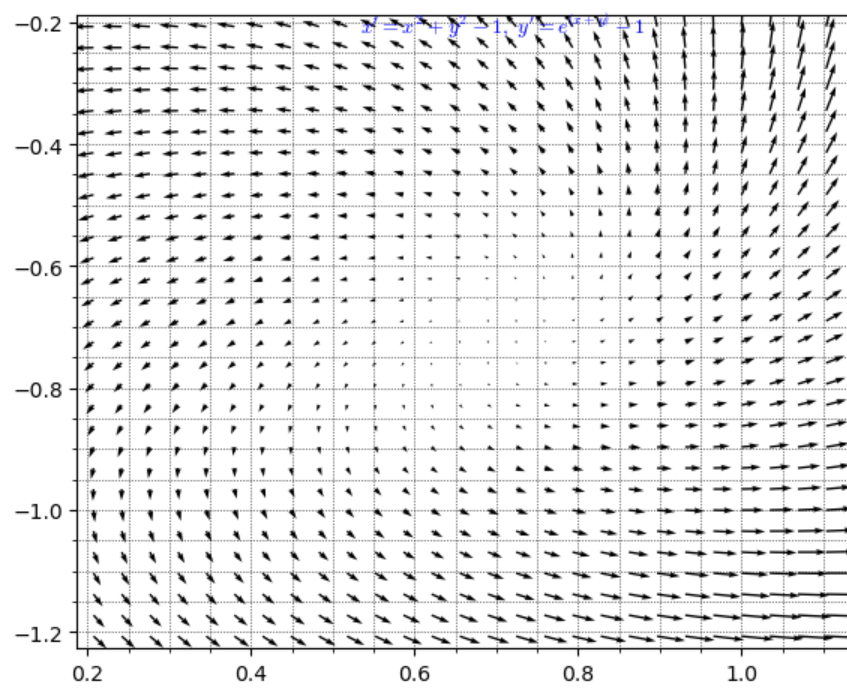
\includegraphics[width=0.3\textwidth]{DU4_1.png}
		\end{center}
		\vspace{-5em}

{\tiny
\begin{verbatim}
var('y')
fx = x^2 + y^2 - 1
fy = exp(x + y) - 1
a = 0.5
p1 = plot_vector_field((fx, fy), (x, sqrt(1/2)-a, sqrt(1/2)+a), (y, -sqrt(1/2)-a, -sqrt(1/2)+a), gridlines='minor', plot_points=30)

p2 = text( r"$x' = %s, \ y' = %s$" %(latex(fx), latex(fy)), (sqrt(1/2), -sqrt(1/2)+a))

total_plot = p1 + p2
total_plot.show()
\end{verbatim}
}


		Okolí druhého ($x = -\sqrt{\frac{1}{2}}$ a $y = \sqrt{\frac{1}{2}}$) je: {\tiny \href{https://sagecell.sagemath.org/?z=eJxVkNEKwjAMRd8F_yHIpCnr1E183J-Io2inhbrWtmj792ZO0L2Um5OQe9On9Mgy48tFn6CFdGqghExvBTWxTEwlh2mkfIKS2G5zWC5cTcoZG7unOkfru14rc0Hsk4A-cwFIogoPH7HeNryS_1Upx4EsYNaft69eX4weVGjZXQ_WMzHZOauHGNr9jmJTjIZiRJUigl8ViVG1DgKOkCdZrGCNRtIEJaOtX5k5B0rwSzR3_6yONkrTjZ7jpTV9gmv-6Sbc7Av5G_OtWfU=&lang=sage&interacts=eJyLjgUAARUAuQ==}{https://sagecell.sagemath.org/?z=eJxVkNEKwjAMRd8F\_yHIpCnr1E183}}\\
		{\tiny \href{https://sagecell.sagemath.org/?z=eJxVkNEKwjAMRd8F_yHIpCnr1E183J-Io2inhbrWtmj792ZO0L2Um5OQe9On9Mgy48tFn6CFdGqghExvBTWxTEwlh2mkfIKS2G5zWC5cTcoZG7unOkfru14rc0Hsk4A-cwFIogoPH7HeNryS_1Upx4EsYNaft69eX4weVGjZXQ_WMzHZOauHGNr9jmJTjIZiRJUigl8ViVG1DgKOkCdZrGCNRtIEJaOtX5k5B0rwSzR3_6yONkrTjZ7jpTV9gmv-6Sbc7Av5G_OtWfU=&lang=sage&interacts=eJyLjgUAARUAuQ==}{J-Io2inhbrWtmj792ZO0L2Um5OQe9On9Mgy48tFn6CFdGqghExvBTWxTEwlh2mkfIKS2G5zWC5cTcoZG7unOkfru14rc0Hsk4A-cwFIogoPH7H}}\\
		{\tiny \href{https://sagecell.sagemath.org/?z=eJxVkNEKwjAMRd8F_yHIpCnr1E183J-Io2inhbrWtmj792ZO0L2Um5OQe9On9Mgy48tFn6CFdGqghExvBTWxTEwlh2mkfIKS2G5zWC5cTcoZG7unOkfru14rc0Hsk4A-cwFIogoPH7HeNryS_1Upx4EsYNaft69eX4weVGjZXQ_WMzHZOauHGNr9jmJTjIZiRJUigl8ViVG1DgKOkCdZrGCNRtIEJaOtX5k5B0rwSzR3_6yONkrTjZ7jpTV9gmv-6Sbc7Av5G_OtWfU=&lang=sage&interacts=eJyLjgUAARUAuQ==}{eNryS\_1Upx4EsYNaft69eX4weVGjZXQ\_WMzHZOauHGNr9jmJTjIZiRJUigl8ViVG1DgKOkCdZrGCNRtIEJaOtX5k5B0rwSzR3\_6yONkrTjZ}}\\
		{\tiny \href{https://sagecell.sagemath.org/?z=eJxVkNEKwjAMRd8F_yHIpCnr1E183J-Io2inhbrWtmj792ZO0L2Um5OQe9On9Mgy48tFn6CFdGqghExvBTWxTEwlh2mkfIKS2G5zWC5cTcoZG7unOkfru14rc0Hsk4A-cwFIogoPH7HeNryS_1Upx4EsYNaft69eX4weVGjZXQ_WMzHZOauHGNr9jmJTjIZiRJUigl8ViVG1DgKOkCdZrGCNRtIEJaOtX5k5B0rwSzR3_6yONkrTjZ7jpTV9gmv-6Sbc7Av5G_OtWfU=&lang=sage&interacts=eJyLjgUAARUAuQ==}{7jpTV9gmv-6Sbc7Av5G\_OtWfU=\&lang=sage\&interacts=eJyLjgUAARUAuQ==}}\\[-2em]

		\begin{center}
			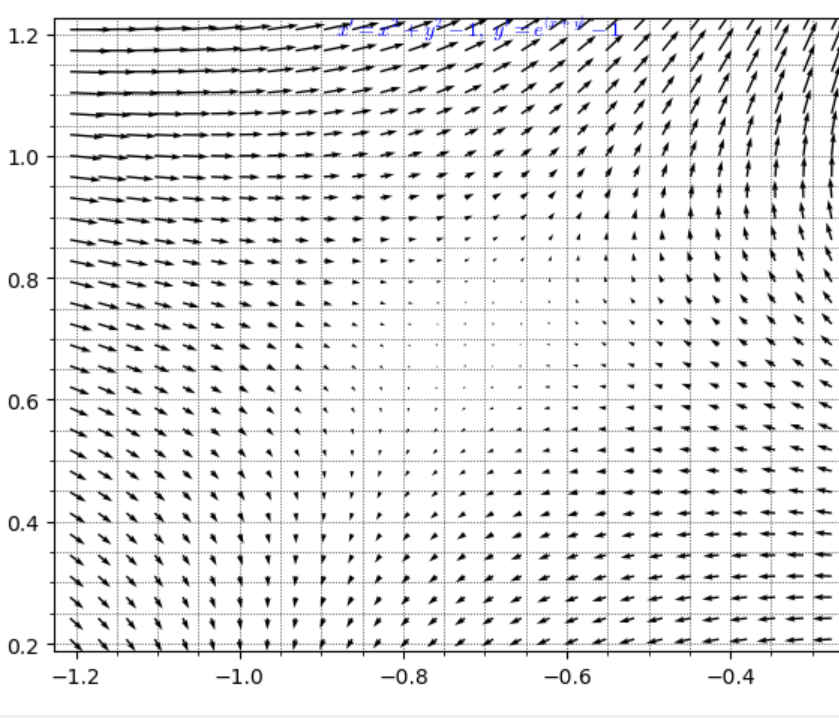
\includegraphics[width=0.3\textwidth]{DU4_2.png}
		\end{center}
		\vspace{-5em}

{\tiny
\begin{verbatim}
var('y')
fx = x^2 + y^2 - 1
fy = exp(x + y) - 1
a = 0.5
p1 = plot_vector_field((fx, fy), (x, -sqrt(1/2)-a, -sqrt(1/2)+a), (y, sqrt(1/2)-a, sqrt(1/2)+a), gridlines='minor', plot_points=30)

p2 = text( r"$x' = %s, \ y' = %s$" %(latex(fx), latex(fy)) , (-sqrt(1/2), sqrt(1/2)+a))

total_plot = p1 + p2
total_plot.show()
\end{verbatim}
}
	\end{reseni}
\end{priklad}

\end{document}
